\documentclass{article}

\usepackage[top=2.5cm, bottom=2.5cm, left=3cm, right=3cm]{geometry}
\usepackage{amsmath,amssymb}

\usepackage{graphicx}
\DeclareGraphicsExtensions{.pdf,.png,.jpg,.mps,.eps,.ps}
\graphicspath{{figs/}}
\usepackage{sidecap} % caption on the side SCfigure

% bold vectors for each alphabet vx
\usepackage{forloop}
\newcommand{\defvec}[1]{\expandafter\newcommand\csname v#1\endcsname{{\mathbf{#1}}}}
\newcounter{ct}
\forLoop{1}{26}{ct}{
    \edef\letter{\alph{ct}}
    \expandafter\defvec\letter
}
\forLoop{1}{26}{ct}{
    \edef\letter{\Alph{ct}}
    \expandafter\defvec\letter
}

\usepackage{bm,xcolor}

\definecolor{goldenbrown}{rgb}{0.5, 0.3, 0.08}
\definecolor{amethyst}{rgb}{0.5, 0.3, 0.7}
\definecolor{awesome}{rgb}{0.9, 0.3, 0.5}
\definecolor{cadmiumgreen}{rgb}{0.0, 0.42, 0.24}

\DeclareMathOperator*{\argmax}{\rm argmax}
\DeclareMathOperator*{\argmin}{\rm argmin}

\newcommand{\inv}{^{-1}}
\newcommand{\trp}{{^\top}} % transpose

\newcommand{\Gaussian}{\ensuremath{\mathcal{N}}} % Gaussian distribution
\newcommand{\inverseLink}{\ensuremath{\textcolor{awesome}{f}}}
\newcommand{\weight}{\vw}
\newcommand{\hyp}{\bm{\theta}}
\newcommand{\likelihood}{\ensuremath{\textcolor{goldenbrown}{p(y|\weight,x,\hyp)}}}
\newcommand{\prior}{\ensuremath{\textcolor{amethyst}{p(\weight|\hyp)}}}
\newcommand{\posterior}{\textcolor{cadmiumgreen}{p(\weight|x,y,\hyp)}}
\begin{document}
\section{General framework for model fitting}
Given $N$ conditioinally independent observations $x = \{(\vx_i)\}, y = \{(y_i)\}$, we want to fit a generic model of the form shown in Fig.~\ref{fig:graphical_model}.
\begin{SCfigure}[\sidecaptionrelwidth][ht]
\centering
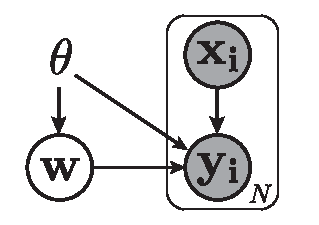
\includegraphics{GLA_graphical_model}
\caption{Graphical model for GLA.
    $\vx_i$ is the independent variable (stimulus), $y_i$ is the dependent variable (output),
    $\weight$ denotes the parameter (weight), and $\hyp$ is the hyperparameter.
    Generalized Linear Awesome (GLA) models have \textbf{linear interaction}
    between the parameter vector $\weight$ and the data $\vx_i$.
}
\label{fig:graphical_model}
\end{SCfigure}
There are two general principles for point estimation that we follow.
\begin{enumerate}
    \item We aim to infer the hyperparameters using evidence optimization (a.k.a. Type-II ML, or empirical Bayes):
	\begin{align}
	    \hyp^\ast = \argmax_{\hyp} p(y|x,\hyp)
		= \argmax_{\hyp} [\log\prior - \log\posterior].
	\end{align}
    \item We aim to infer the \textit{maximum a posteriori} (MAP) parameters given the hyperparameter:
	\begin{align}
	    \weight^\ast = \argmax_{\weight} \posterior =
		\argmax_{\weight} \left[ \log\likelihood + \log\prior \right].
	\end{align}
\end{enumerate}
Depending on the likelihood and prior, we need approximations and numerical tricks to achieve our goals.

\section{Likelihoods}
We support three basic types of observation models.
\begin{align}
    \log\likelihood &= 
	-\frac{N}{2}\log2\pi\textcolor{red}{\sigma^2}
	- \frac{1}{2\textcolor{red}{\sigma^2}} 
	\sum_i
	    (\inverseLink(\weight\trp\vx_i) - y_i)\trp
	    (\inverseLink(\weight\trp\vx_i) - y_i) 
	\qquad 
	&\text{\it Gaussian}
    \label{eq:likelihood:Gaussian}
    \\
    \log\likelihood &= 
	\sum_i y_i \log \inverseLink(\weight\trp\vx_i)
	-
	\sum_i \inverseLink(\weight\trp\vx_i)
	+ \sum_i y_i!
	\qquad 
	&\text{\it Poisson}
    \label{eq:likelihood:Poisson}
    \\
    \log\likelihood &= 
	\sum_i
	y_i \log\inverseLink(\weight\trp\vx_i)
	+
	\sum_i
	(1-y_i) \log (1-\inverseLink(\weight\trp\vx_i))
	\qquad
	&\text{\it Bernoulli}
    \label{eq:likelihood:Bernoulli}
    \\
    \log\likelihood &= 
	\sum_i
	y_i \log\inverseLink(\weight\trp\vx_i) 
	- \textcolor{red}{\nu} \sum_i \log y_i!
	- \log Z(\inverseLink(\weight\trp\vx_i), \textcolor{red}{\nu})
	&\text{\it COM-Poisson}
    \label{eq:likelihood:COM}
\end{align}
where $\textcolor{red}{\sigma^2}$ is the variance for the Gaussian observations, and $\inverseLink$ is the inverse link function.
$\textcolor{red}{\sigma^2}$ and $\textcolor{red}{\nu}$ are included as hyperparameters in $\hyp$ for the purpose of fitting, though it is not a part of the prior.
COM-Poisson stands for {\it Conway-Maxwell-Poisson} distribution which generalizes Poisson distribution to handle both underdispersion and overdispersion.

\section{Priors}
We mainly support Gaussian priors.
\begin{align}
    \log\prior =
	-\frac{1}{2}\log|2\pi C(\hyp)| 
	-\frac{1}{2}(\weight - \vb)\trp C(\hyp)\inv (\weight - \vb)
	\label{eq:prior:Gaussian}
\end{align}
where $C(\hyp)$ is the covariance matrix, and $\vb$ is the mean vector, both parameterized by hyperparameters in $\hyp$.
In most cases, $\vb = 0$.
The form and parameterization of $C(\hyp)$ can be quite diverse and achieve regularization, sparsification, smoothness with aid of evidence optimization.
Here are some examples:
\begin{align}
    C(\hyp) &= \textcolor{red}{\rho} \vI \qquad & \text{\it Ridge}
    \label{eq:prior:Ridge}
    \\
    C(\hyp)\inv &= \begin{bmatrix} 
		    \textcolor{red}{\alpha_1} & 0        & \cdots& \\
		    0        & \textcolor{red}{\alpha_2} & \cdots & \\
		    \vdots   & \vdots   & \ddots & \\
		    &          & 0      & \textcolor{red}{\alpha_d} \\
		\end{bmatrix}
	    \qquad & \text{\it Automatic Relevance Determination (ARD)}
    \label{eq:prior:ARD}
    \\
    C(\hyp)_{i,j} &= \exp(-\textcolor{red}{\rho} -d(i,j)^2/2\textcolor{red}{\delta}^2 )
	    \qquad & \text{\it Automatic Smoothness Determination (ASD)}
    \label{eq:prior:ASD}
\end{align}

Often the stimulus is concatenation of independent sources, and hence pieces of the weight vector $\weight$ require separate hyperparameters which results in a block diagonal $C(\hyp)$ (and $C(\hyp)\inv$).

\section{Posterior inference}
\subsection{Gaussian likelihood}
For gaussian likelihood and identity inverse link, the posterior is Guassian, straightforward, and familiar.
\begin{align}
    \posterior &= \Gaussian(\mu, \Lambda)
    \label{eq:posterior:Gaussian}
    \\
    \mu &= \frac{1}{\sigma^2}\Lambda \sum_i \vx_i y_i\\
    \Lambda &= \left(\frac{1}{\sigma^2}\sum_i \vx_i \vx_i\trp + C(\hyp)\inv\right)\inv
\end{align}

\subsection{General case}
Since Gaussian prior is not conjugate for other likelihoods, typically a MAP solution is obtained by numerical optimization.
The simplest Gaussian approximation of the posterior is to use the Laplace approximation: set the mean as the MAP solution, and use the (negative) Hessian of the log-posterior at MAP as the inverse covariance.
\begin{align}
    \posterior &\simeq \Gaussian(\mu, \Lambda)
    \label{eq:posterior:Laplace}
    \\
    \mu &= \weight^\ast
    \\
    \Lambda\inv &= 
	\left.
	-\frac{\partial^2}{\partial \weight \partial \weight}
	\log \posterior \right\vert_{\weight = \weight^\ast}
	\\
	&=
	\left.
	-\frac{\partial^2}{\partial \weight \partial \weight}
	\left[ \log\likelihood + \log\prior \right]
	\right\vert_{\weight = \weight^\ast}
	\\
	&=
	\left.
	-\frac{\partial^2}{\partial \weight \partial \weight}
	\log\likelihood
	\right\vert_{\weight = \weight^\ast}
	+ C(\hyp)\inv
\end{align}

\section{Evidence optimization}

\end{document}
